\chapter{Qt GUI Screenshots}
\label{appendix:qt-gui-screenshots}

\begin{figure}[h!]
	\centering
	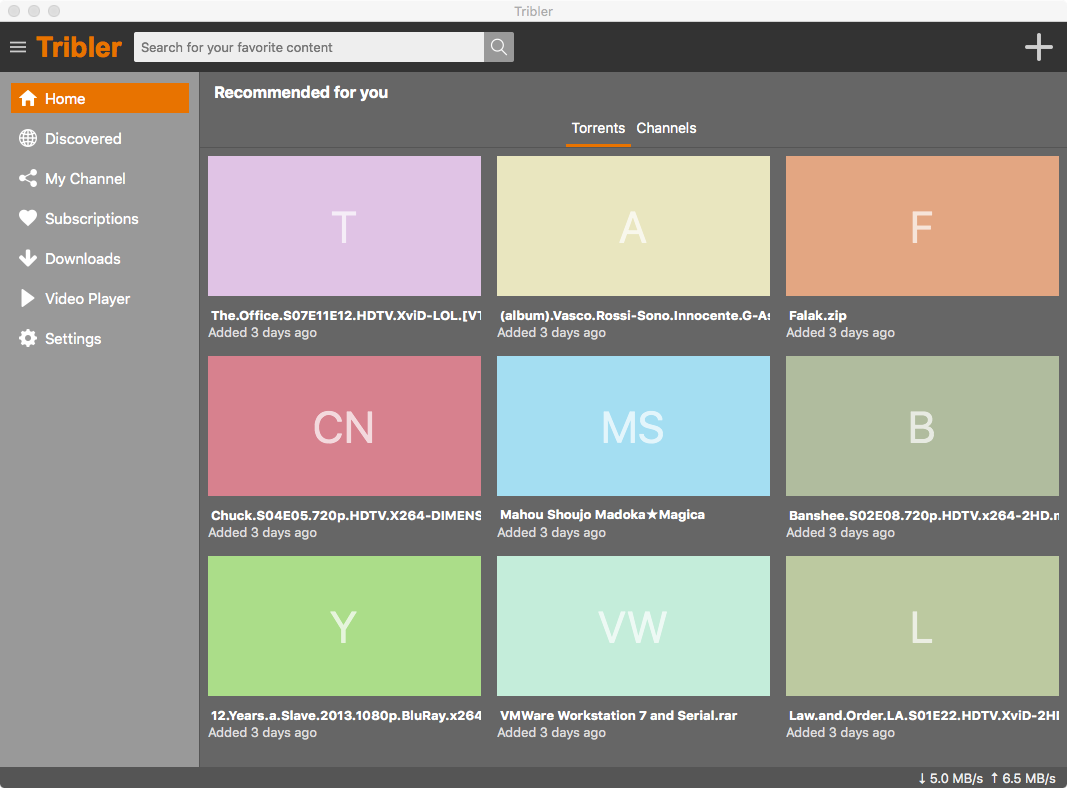
\includegraphics[width=0.95\columnwidth]{images/qt_gui/screenshot_homepage}
	\caption{The homepage of the Qt GUI.}
	\label{fig:gui-screenshot-homepage}
\end{figure}

\begin{figure}[h!]
	\centering
	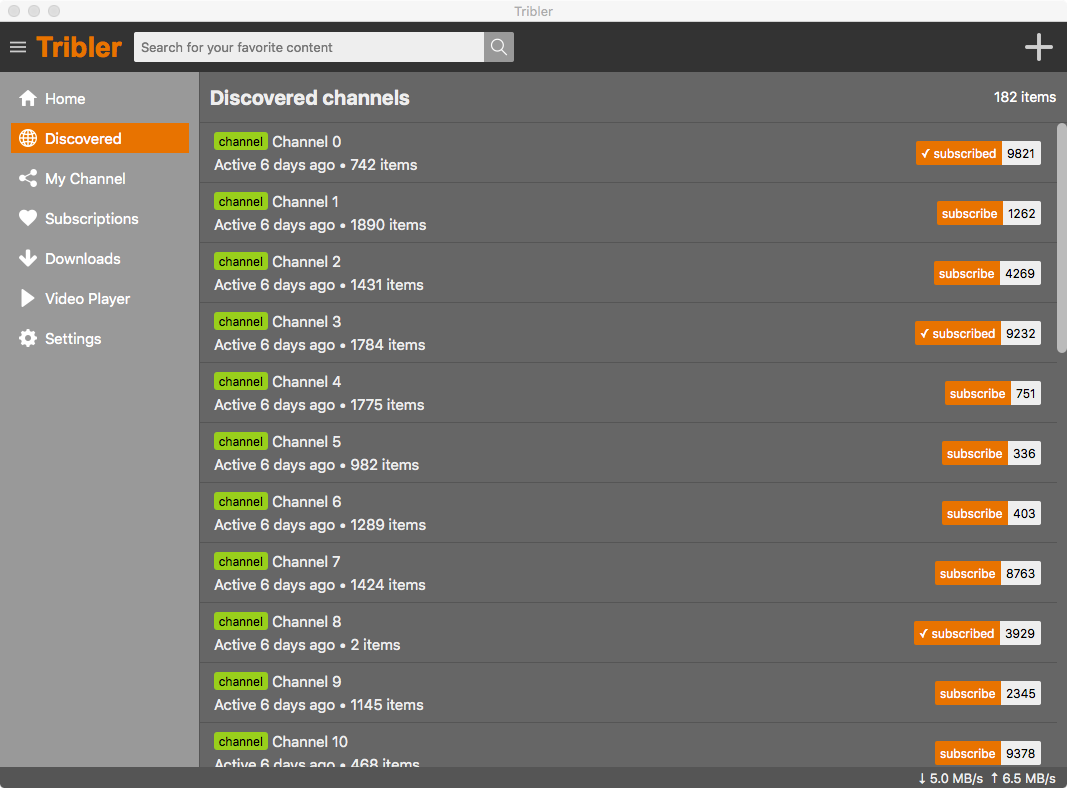
\includegraphics[width=0.95\columnwidth]{images/qt_gui/screenshot_discovered}
	\caption{The page with discovered channels.}
	\label{fig:gui-screenshot-discovered}
\end{figure}

\begin{figure}[h!]
	\centering
	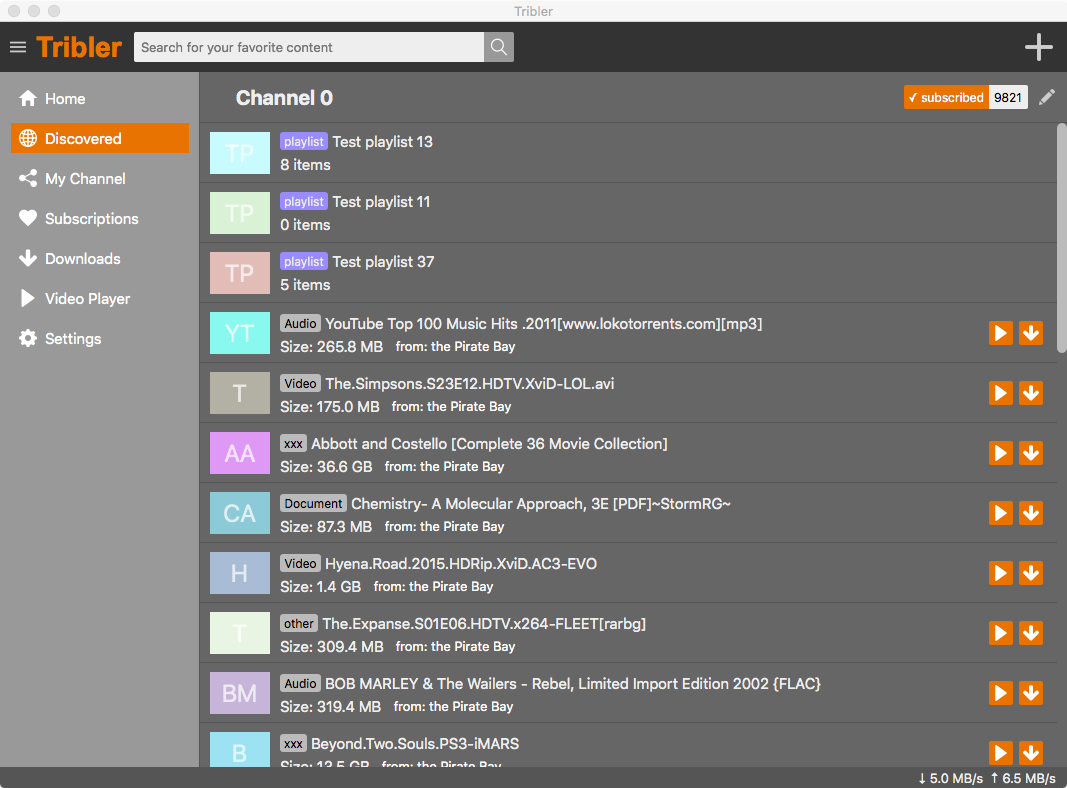
\includegraphics[width=0.95\columnwidth]{images/qt_gui/screenshot_channel}
	\caption{The page that presents content in a specific channel.}
	\label{fig:gui-screenshot-channel}
\end{figure}

\begin{figure}[h!]
	\centering
	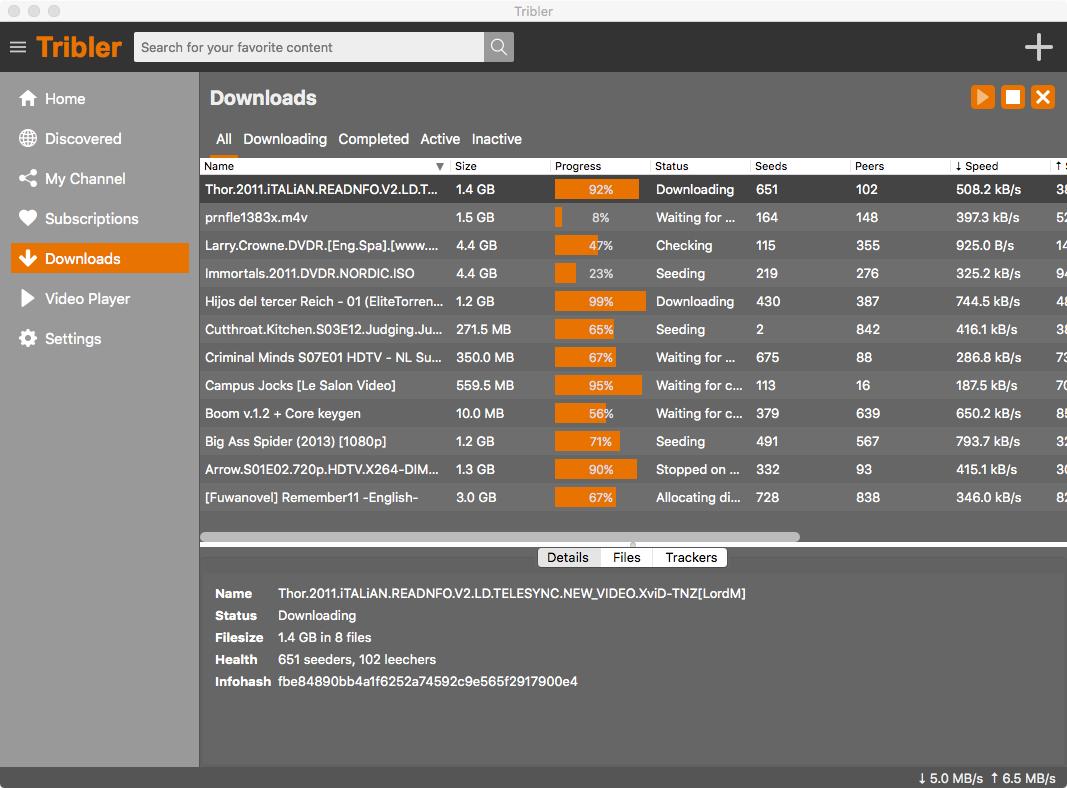
\includegraphics[width=0.95\columnwidth]{images/qt_gui/screenshot_downloads}
	\caption{The overview page of the downloads.}
	\label{fig:gui-screenshot-downloads}
\end{figure}

\begin{figure}[h!]
	\centering
	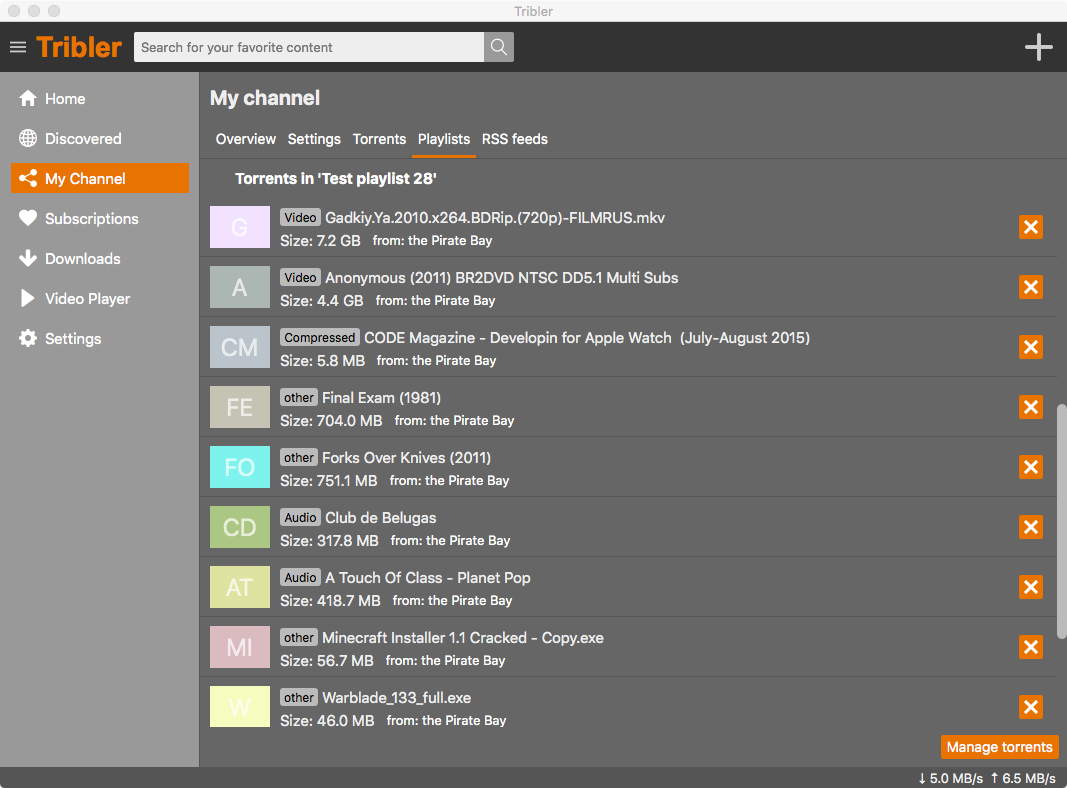
\includegraphics[width=0.95\columnwidth]{images/qt_gui/screenshot_my_channel}
	\caption{The page where one can manage playlists in an owned channel.}
	\label{fig:gui-screenshot-my-channel}
\end{figure}

\begin{figure}[h!]
	\centering
	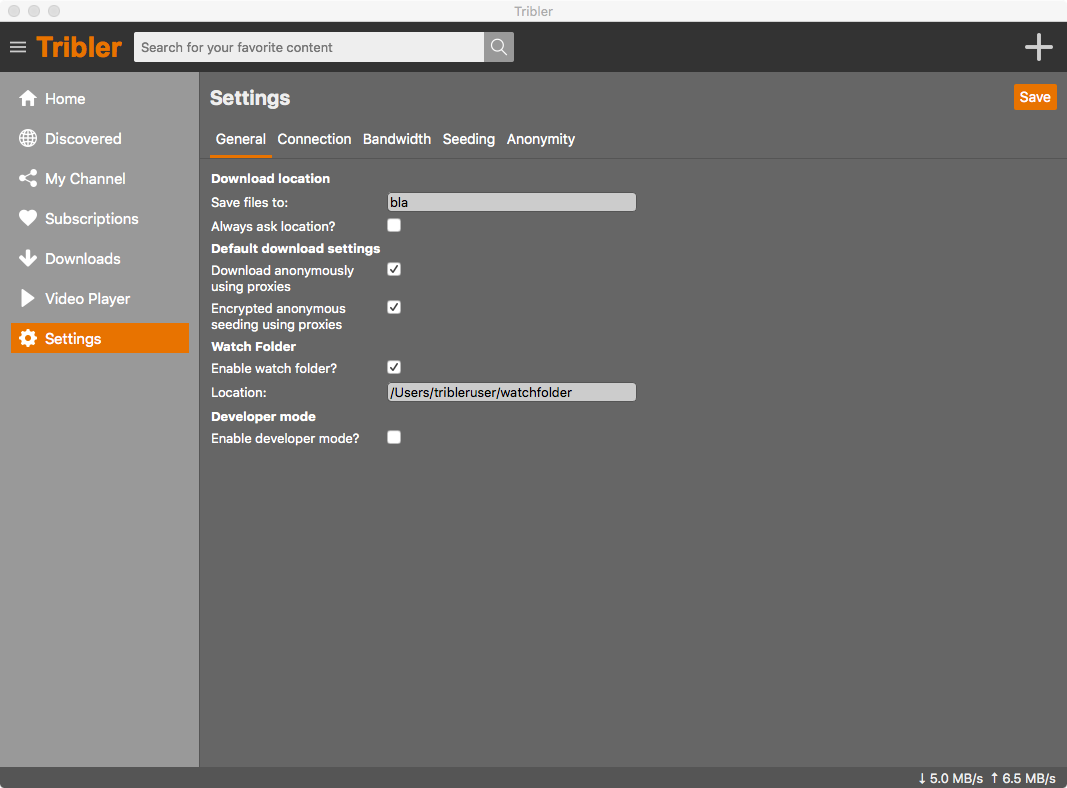
\includegraphics[width=0.95\columnwidth]{images/qt_gui/screenshot_settings}
	\caption{The settings page.}
	\label{fig:gui-screenshot-settings}
\end{figure}

\begin{figure}[h!]
	\centering
	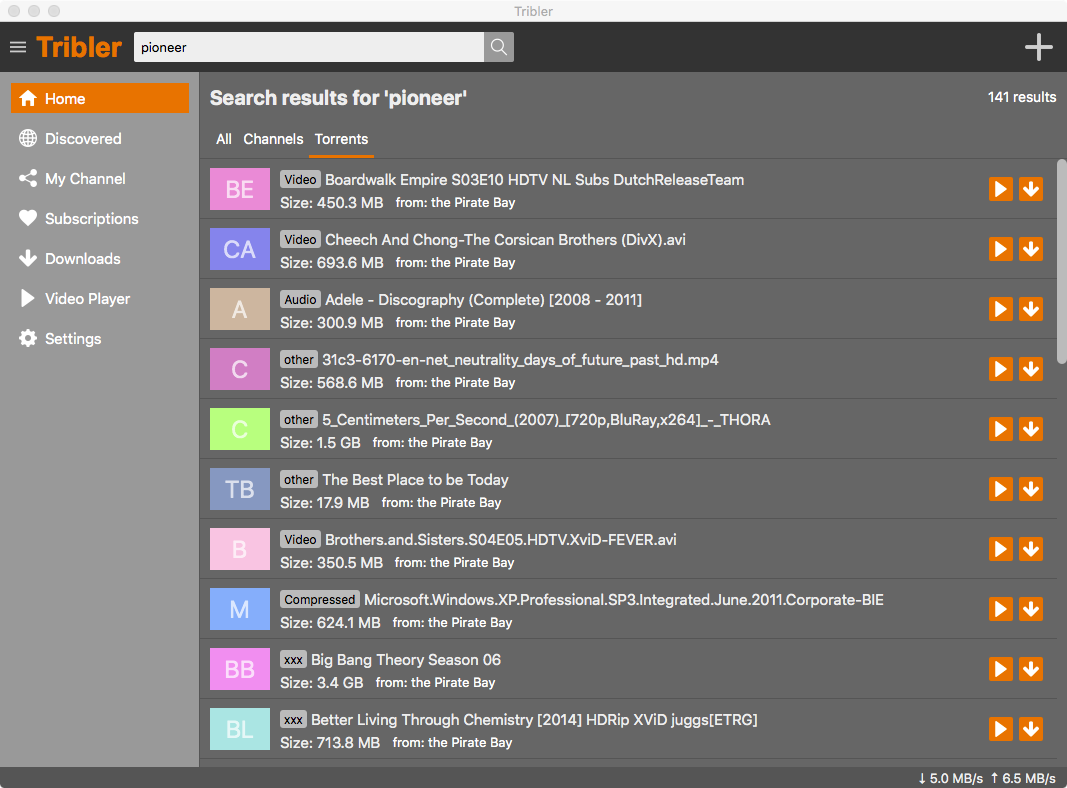
\includegraphics[width=0.95\columnwidth]{images/qt_gui/screenshot_search_results}
	\caption{The page with (mocked) search results.}
	\label{fig:gui-screenshot-search-results}
\end{figure}